\chapter{Example Models}
\label{example_models}

In this chapter, two ACT-R models are translated into CHR and the results are discussed. The examples are taken from \citetitle{actr_tutorial} \cite{actr_tutorial}.

\section{The Counting Model}

The first model is an extension of the example presented in section~\ref{example_counting}. The code has been published in unit 1 of \citetitle{actr_tutorial} \cite{actr_tutorial} as shipped with the source code of the vanilla ACT-R 6.0 implementation. Basically, the counting process is modeled by a set of static facts that a person has learned and retrieves for the counting process from declarative memory. The following model definition is discussed:

\begin{lstlisting}[escapeinside={(*@}{@*)}, caption={ACT-R code of the counting example}, label=exmod:lst:example_counting]
(define-model count (*@\label{exmod:lst:example_counting:define_model}@*)

(chunk-type count-order first second) (*@\label{exmod:lst:example_counting:chunk_type}@*)
(chunk-type count-from start end count)

(add-dm (*@\label{exmod:lst:example_counting:add_dm}@*)
 (b ISA count-order first 1 second 2)
 (c ISA count-order first 2 second 3)
 (d ISA count-order first 3 second 4)
 (e ISA count-order first 4 second 5)
 (f ISA count-order first 5 second 6)
 (first-goal ISA count-from start 2 end 4)
 ) (*@\label{exmod:lst:example_counting:add_dm_end}@*)

(p start (*@\label{exmod:lst:example_counting:start}@*)
   =goal>
      ISA         count-from
      start       =num1
      count       nil
 ==>
   =goal>
      count       =num1
   +retrieval>
      ISA         count-order
      first       =num1
)

(P increment (*@\label{exmod:lst:example_counting:increment}@*)
   =goal>
      ISA         count-from
      count       =num1
    - end         =num1
   =retrieval>
      ISA         count-order
      first       =num1
      second      =num2
 ==>
   =goal>
      count       =num2
   +retrieval>
      ISA         count-order
      first       =num2
   !output!       (=num1)
)

(P stop (*@\label{exmod:lst:example_counting:stop}@*)
   =goal>
      ISA         count-from
      count       =num
      end         =num
 ==>
   -goal>
   !output!       (=num)
)

(goal-focus first-goal) (*@\label{exmod:lst:example_counting:goal_focus}@*)
)
\end{lstlisting}

First of all, in line~\ref{exmod:lst:example_counting:define_model} the model definition is initiated and a model name is given. Line~\ref{exmod:lst:example_counting:chunk_type} sq. add the two necessary chunk-types: A chunk-type for the goal-chunks and a chunk-type for the actual declarative data. These chunk-type definitions are global to the system, i.e. they are added to all chunk stores. The goal-chunks have the slots \lstinline|start| and \lstinline|end| which encode from which number the counting process should start and where it should end. The value in the slot \lstinline|count| saves the current number of the count-process, analogously as in section~\ref{example_counting}. Then the chunks are added from line~\ref{exmod:lst:example_counting:add_dm} to~\ref{exmod:lst:example_counting:add_dm_end} and are representations of the order of the natural numbers from one to six. The last chunk is the goal-chunk. Note that only the start and end numbers are specified, the current number will be set to \lstinline|nil|.

The first production rule \lstinline|start| in line~\ref{exmod:lst:example_counting:start} sqq. can only be applied, if the goal has an empty \lstinline|count| slot, but an actual value in the \lstinline|start| slot. This will be valid for the initial state as explained later. The production states a request for the first count-fact with the start number in its \lstinline|first| slot and sets the current number in the goal to the start number. The other slots in the goal buffer remain the same.

In line~\ref{exmod:lst:example_counting:increment} sqq. the main rule \lstinline|increment| is defined. It assumes that a count-order fact which matches the current number in the goal has been retrieved. Additionally, the counting process must not end with this number, indicated by the negated slot test on the slot \lstinline|end|. The action part then states a new request for the next count-fact and increments the current number. Once the rule is applicable, it will be applicable as long there are count-facts in the declarative memory and the specified end has not been reached, yet.

The last production rule \lstinline|stop| in line~\ref{exmod:lst:example_counting:stop} is applicable, as soon the \lstinline|increment| rule cannot be applied anymore due to the fact that the specified end of the counting process has been reached. Then, the last number will be printed and the goal buffer will be cleared.

The last function call in line~\ref{exmod:lst:example_counting:goal_focus} is an initialization method, which simply puts the previously defined chunk \lstinline|first-goal| into the goal buffer. This leads to an initial state where the rule \lstinline|start| is applicable.

The output of the model is:

\begin{lstlisting}
     0.000   GOAL             SET-BUFFER-CHUNK GOAL FIRST-GOAL 
     0.000   PROCEDURAL       CONFLICT-RESOLUTION 
     0.050   PROCEDURAL       PRODUCTION-FIRED START 
     0.050   PROCEDURAL       CLEAR-BUFFER RETRIEVAL 
     0.050   DECLARATIVE      START-RETRIEVAL 
     0.050   DECLARATIVE      RETRIEVED-CHUNK C 
     0.050   DECLARATIVE      SET-BUFFER-CHUNK RETRIEVAL C 
     0.050   PROCEDURAL       CONFLICT-RESOLUTION 
     0.100   PROCEDURAL       PRODUCTION-FIRED INCREMENT 
2 
     0.100   PROCEDURAL       CLEAR-BUFFER RETRIEVAL 
     0.100   DECLARATIVE      START-RETRIEVAL 
     0.100   DECLARATIVE      RETRIEVED-CHUNK D 
     0.100   DECLARATIVE      SET-BUFFER-CHUNK RETRIEVAL D 
     0.100   PROCEDURAL       CONFLICT-RESOLUTION 
     0.150   PROCEDURAL       PRODUCTION-FIRED INCREMENT 
3 
     0.150   PROCEDURAL       CLEAR-BUFFER RETRIEVAL 
     0.150   DECLARATIVE      START-RETRIEVAL 
     0.150   DECLARATIVE      RETRIEVED-CHUNK E 
     0.150   DECLARATIVE      SET-BUFFER-CHUNK RETRIEVAL E 
     0.150   PROCEDURAL       CONFLICT-RESOLUTION 
     0.200   PROCEDURAL       PRODUCTION-FIRED STOP 
4 
     0.200   PROCEDURAL       CLEAR-BUFFER GOAL 
     0.200   PROCEDURAL       CONFLICT-RESOLUTION 
     0.200   ------           Stopped because no events left to process 
\end{lstlisting}

The source file in listing \ref{exmod:lst:example_counting} can be translated by the provided CHR compiler which yields the following result:

\begin{lstlisting}[escapeinside={(*@}{@*)}, caption={Auto-generated CHR code of the counting example}, label=exmod:lst:example_counting_chr]
:- include('actr_core.pl').
:- chr_constraint run/0, fire/0.

delay-start @ 
  fire,
  buffer(goal,_,A),
    chunk(A,count-from),
    chunk_has_slot(A,start,B),
    chunk_has_slot(A,count,nil)
==>
  B\==nil |
  conflict_set(start).

start @ 
  buffer(goal,_,A),
    chunk(A,count-from),
    chunk_has_slot(A,start,B),
    chunk_has_slot(A,count,nil)
  \ apply_rule(start)
<=>
  B\==nil |
  buffer_change(goal,chunk(_,_,[ (count,B)])),
  buffer_request(retrieval,chunk(_,count-order,[ (first,B)])),
  conflict_resolution.

delay-increment @ 
  fire,
  buffer(goal,_,A),
    chunk(A,count-from),
    chunk_has_slot(A,count,C),
    chunk_has_slot(A,end,D),
  buffer(retrieval,_,B),
    chunk(B,count-order),
    chunk_has_slot(B,first,C),
    chunk_has_slot(B,second,E)
==>
  C\==nil,
  D\==C,
  E\==nil |
  conflict_set(increment).

increment @ 
  buffer(goal,_,A),
    chunk(A,count-from),
    chunk_has_slot(A,count,C),
    chunk_has_slot(A,end,D),
  buffer(retrieval,_,B),
    chunk(B,count-order),
    chunk_has_slot(B,first,C),
    chunk_has_slot(B,second,E)
  \ apply_rule(increment)
<=>
  C\==nil,
  D\==C,
  E\==nil |
  buffer_change(goal,chunk(_,_,[ (count,E)])),
  buffer_request(retrieval,chunk(_,count-order,[ (first,E)])),
  output(C),
  conflict_resolution.

delay-stop @
  fire,
  buffer(goal,_,A),
    chunk(A,count-from),
    chunk_has_slot(A,count,B),
    chunk_has_slot(A,end,B)
==>
  B\==nil | 
  conflict_set(stop).

stop @ 
  buffer(goal,_,A),
    chunk(A,count-from),
    chunk_has_slot(A,count,B),
    chunk_has_slot(A,end,B)
  \ apply_rule(stop)
<=>
  B\==nil |
  buffer_clear(goal),
  output(B),
  conflict_resolution.
  
init @ (*@\label{exmod:lst:example_counting_chr:init}@*)
run <=> true | 
  set_default_utilities([stop,increment,start]),
  add_buffer(retrieval,declarative_module),
  add_buffer(goal,declarative_module),
  lisp_chunktype([chunk]),
  lisp_chunktype([count-order,first,second]),
  lisp_chunktype([count-from,start,end,count]),
  lisp_adddm([[b,isa,count-order,first,1,second,2],
    [c,isa,count-order,first,2,second,3],
    [d,isa,count-order,first,3,second,4],
    [e,isa,count-order,first,4,second,5],
    [f,isa,count-order,first,5,second,6],
    [first-goal,isa,count-from,start,2,end,4]]),
  lisp_goalfocus([first-goal]),
  now(0),
  conflict_resolution,
  nextcyc.
  
no-rule @ (*@\label{exmod:lst:example_counting_chr:no_rule}@*)
fire <=> true |
  conflict_set([]),
  choose.
\end{lstlisting}

First of all, it is interesting to note, that there are some more CHR rules than production rules in the original code in listing~\ref{exmod:lst:example_counting}. One very obvious extension is the rule \lstinline|init| in line~\ref{exmod:lst:example_counting_chr:init}. This rule initializes the model according to section~\ref{initialization}. First, it sets the default utilities for each of the production rules and creates the used buffers in the buffer system. Then, the Lisp functions from the original model definitions are called in their CHR versions, according to section~\ref{lisp_functions}. Those are the methods which create chunk-types and add the initial declarative knowledge to the declarative module. Note that also the artificial chunk-type \lstinline|chunk| with no slots is created. The last Lisp call moves the \lstinline|first-goal| chunk to the goal buffer. Finally, the current time is set to zero, a conflict resolution event is scheduled in the queue (according to section~\ref{implementation:conflict_resolution}) and the recognize-act cycle is started by \lstinline|nextcyc|, which will dequeue the first event from the scheduler as described in section~\ref{implementation:scheduler:recognize-act}.

Furthermore, each production rule from the original module has two correspondent CHR rules in the translation due to the conflict resolution process described in section~\ref{implementation:conflict_resolution}. The first rule delays the execution by adding the rule -- if applicable -- to the conflict set as soon as a new conflict resolution event (represented by the CHR constraint \lstinline|fire|) has been triggered. The second rule actually performs the rule, if it has been chosen by the conflict resolution process (indicated by the constraint \lstinline|apply_rule/1|). After the rule application, each rule schedules the next conflict resolution event by adding \lstinline|conflict_resolution| to the store. The guards of the production rules check that each tested slot actually has a value (so its value is not \lstinline|nil|) as described in section~\ref{empty_slots} (see page~\pageref{empty_slots}) and in the rule \lstinline|increment|, for example, a negated slot test is translated to a guard check according to the pattern presented in section~\ref{slot_modifiers} (see page~\pageref{slot_modifiers}).

The rule \lstinline|no-rule| in line~\ref{exmod:lst:example_counting_chr:no_rule} is the last rule tested in the collecting process of the conflict resolution. It removes the \lstinline|fire| constraint and triggers the choosing process, after it has added an empty rule to the conflict set. This is important for the choosing process to detect if no rule was applicable in this conflict resolution phase.

The output of the model is the following (pretty printed by hand):

\begin{lstlisting}
?- run.
0      ... calling event: do_conflict_resolution
           going to apply rule start
0.05   ... calling event: apply_rule(start)
           firing rule start
0.05   ... calling event: do_buffer_change(goal,chunk(_G17029,_G17030,[ (count,2)]))
0.05   ... calling event: start_request(retrieval,chunk(_G17476,count-order,[ (first,2)]))
           Started buffer request retrieval
           clear buffer retrieval
0.05   ... calling event: do_conflict_resolution
           No rule matches -> Schedule next conflict resolution event
1.05   ... calling event: do_buffer_request(retrieval,chunk(_G17476,count-order,[ (first,2)]))
           Retrieved chunk c
           Put chunk c into buffer
1.05   ... calling event: do_conflict_resolution
           going to apply rule increment
1.1:0  ... calling event: apply_rule(increment)
           firing rule increment
output:2
1.1    ... calling event: do_buffer_change(goal,chunk(_G33694,_G33695,[ (count,3)]))
1.1    ... calling event: start_request(retrieval,chunk(_G34139,count-order,[ (first,3)]))
           Started buffer request retrieval
           clear buffer retrieval
1.1    ... calling event: do_conflict_resolution
           No rule matches -> Schedule next conflict resolution event
2.1    ... calling event: do_buffer_request(retrieval,chunk(_G34139,count-order,[ (first,3)]))
           Retrieved chunk d
           Put chunk d into buffer
2.1    ... calling event: do_conflict_resolution
           going to apply rule increment
2.15   ... calling event: apply_rule(increment)
           firing rule increment
output:3
2.15   ... calling event: do_buffer_change(goal,chunk(_G25849,_G25850,[ (count,4)]))
2.15   ... calling event: start_request(retrieval,chunk(_G26294,count-order,[ (first,4)]))
           Started buffer request retrieval
           clear buffer retrieval
2.15   ... calling event: do_conflict_resolution
           going to apply rule stop
2.1999 ... calling event: apply_rule(stop)
           firing rule stop
output:4
2.1999 ... calling event: do_buffer_clear(goal)
           clear buffer goal
2.1999 ... calling event: do_conflict_resolution
           No rule matches -> Schedule next conflict resolution event
3.15   ... calling event: do_buffer_request(retrieval,chunk(_G26294,count-order,[ (first,4)]))
           performing request: retrieval
           Retrieved chunk e
           Put chunk e into buffer
3.15   ... calling event: do_conflict_resolution
           No rule matches -> Schedule next conflict resolution event
           No more events in queue. End of computation.
\end{lstlisting}

Note that the output is very similar to the original output, especially the order of rule applications and events. However, the timings are not accurate, yet, since some constants are different from the original implementation, which can be fixed and does not really harm the theory. 

To demonstrate the subsymbolic layer, the original code is extended as follows:

\begin{lstlisting}[escapeinside={(*@}{@*)}]
(define-model count

(sgp :esc t)


(chunk-type count-order first second)
(chunk-type goal-chunk goal start end count)

(add-dm
 ...
 (d ISA count-order first 3 second 4)
 (d1 ISA count-order first 3 second 5)
 ...
 (second-goal ISA goal-chunk goal training1)
 )
 
(p train1
  =goal>
    ISA           goal-chunk
    goal          training1
 ==>
  =goal>
    goal          training2
  +retrieval>
    ISA           count-order
    first         3
    second        4
)

(p train2
  =goal>
    ISA           goal-chunk
    goal          training2
  =retrieval>
    ISA           count-order
    first         3
    second        4
 ==>
  =goal>
    ISA           goal-chunk
    start         2
    end           4
    goal          count
  -retrieval> 
)
 
(p start
    { defined as in listing (*@\ref{exmod:lst:example_counting}@*) }
)

(P increment
  { defined as in listing (*@\ref{exmod:lst:example_counting}@*) }
)

(P incrementx
   =goal>
      ISA         goal-chunk
      goal        count
      count       =num1
    - end         =num1
   =retrieval>
      ISA         count-order
      first       =num1
      second      =num2
 ==>
   -goal>
   !output!       (wrong)
)

(P stop
   { defined as in listing (*@\ref{exmod:lst:example_counting}@*) }

)

(goal-focus second-goal)

(spp increment :u 8 incrementx :u 0)
(spp stop :reward 15)
)
\end{lstlisting}

The subsymbolic layer is turned on and chunk \lstinline|d1| which encodes a false count fact is added. Additionally, there are two training rules, which just retrieve the fact \lstinline|d| to increase its activity and then reset the state to the initial state of the model in listing~\ref{exmod:lst:example_counting}. The goal is set to a chunk, which leads the first training rule to match at first. Furthermore, a broken rule which matches the same context as the original \lstinline|increment| rule is added. The initial utility of the correct \lstinline|increment| rule is set to 8, whereas the corrupted rule gets an initial value of 0. Additionally, the reward the rule \lstinline|stop| can distribute, is set to 15, so the reaching of the final state is rewarded and all rules which lead to that state get a certain amount of this reward. The full code can be found in appendix~\ref{app:ex:subsymbolic_layer}. 

When executing the resulting CHR model, this yields the following output (times have been cut after four digits):

\begin{lstlisting}
?- run.
0      ... calling event: do_conflict_resolution
           going to apply rule train1
0.05   ... calling event: apply_rule(train1)
           firing rule train1
0.05   ... calling event: do_buffer_change(goal,chunk(_G26126,_G26127,[ (goal,training2)]))
0.05   ... calling event: start_request(retrieval,chunk(_G26573,count-order,[ (first,3), (second,4)]))
           Started buffer request retrieval
           clear buffer retrieval:nil
0.05   ... calling event: do_conflict_resolution
           No rule matches -> Schedule next conflict resolution event
0.0974 ... calling event: do_buffer_request(retrieval,chunk(_G26573,count-order,[ (first,3), (second,4)]))
           performing request: retrieval
           Retrieved chunk d
           Put chunk d into buffer
0.0974 ... calling event: do_conflict_resolution
           going to apply rule train2
0.1474 ... calling event: apply_rule(train2)
           firing rule train2
0.1474 ... calling event: do_buffer_change(goal,chunk(_G44291,goal-chunk,[ (start,2), (end,4), (goal,count)]))
0.1474 ... calling event: do_buffer_clear(retrieval)
           clear buffer retrieval:d
0.1474 ... calling event: do_conflict_resolution
           going to apply rule start
0.1974 ... calling event: apply_rule(start)
           firing rule start
0.1974 ... calling event: do_buffer_change(goal,chunk(_G26238,_G26239,[ (count,2)]))
0.1974 ... calling event: start_request(retrieval,chunk(_G26683,count-order,[ (first,2)]))
           Started buffer request retrieval
           clear buffer retrieval:nil
0.1974 ... calling event: do_conflict_resolution
           No rule matches -> Schedule next conflict resolution event
0.2575 ... calling event: do_buffer_request(retrieval,chunk(_G26683,count-order,[ (first,2)]))
           performing request: retrieval
           Retrieved chunk c
           Put chunk c into buffer
0.2575 ... calling event: do_conflict_resolution
           going to apply rule increment
0.3075 ... calling event: apply_rule(increment)
           firing rule increment
output:2
0.3075 ... calling event: do_buffer_change(goal,chunk(_G44015,_G44016,[ (count,3)]))
0.3075 ... calling event: start_request(retrieval,chunk(_G44460,count-order,[ (first,3)]))
           Started buffer request retrieval
           clear buffer retrieval:c
0.3075 ... calling event: do_conflict_resolution
           No rule matches -> Schedule next conflict resolution event
0.3657 ... calling event: do_buffer_request(retrieval,chunk(_G44460,count-order,[ (first,3)]))
           performing request: retrieval
           Retrieved chunk d
           Put chunk d into buffer
0.3657 ... calling event: do_conflict_resolution
           going to apply rule increment
0.4157 ... calling event: apply_rule(increment)
           firing rule increment
output:3
0.4157 ... calling event: do_buffer_change(goal,chunk(_G68222,_G68223,[ (count,4)]))
0.4157 ... calling event: start_request(retrieval,chunk(_G68667,count-order,[ (first,4)]))
           Started buffer request retrieval
           clear buffer retrieval:d
0.4157 ... calling event: do_conflict_resolution
           going to apply rule stop
0.4657 ... calling event: apply_rule(stop)
           firing rule stop
           triggered reward for rule: stop
           triggered reward for rule: increment
           triggered reward for rule: increment
           triggered reward for rule: start
           triggered reward for rule: train2
           triggered reward for rule: train1
           reward triggered by rule stop
output:4
0.4657 ... calling event: do_buffer_clear(goal)
           clear buffer goal:first-goal
0.4657 ... calling event: do_conflict_resolution
           No rule matches -> Schedule next conflict resolution event
0.5029 ... calling event: do_buffer_request(retrieval,chunk(_G36175,count-order,[ (first,4)]))
           performing request: retrieval
           Retrieved chunk e
           Put chunk e into buffer
0.5029 ... calling event: do_conflict_resolution
           No rule matches -> Schedule next conflict resolution event
           No more events in queue. End of computation.
\end{lstlisting}

Due to the training of chunk~\lstinline|d| which increased the activation of this chunk according to the base-level learning equation, the other matching chunk \lstinline|d1| is not being retrieved in the computational process.

Furthermore, the rule \lstinline|increment| is applied instead of \lstinline|incrementx|, although both are matching the context, due to the higher intitial utility value of \lstinline|increment|. The reward of the rule stop leads to the following utilities at the end of the computation (taken from the final CHR store):

\begin{lstlisting}
production_utility(train1,6.916852474603892)
production_utility(train2,6.9363461811027785)
production_utility(start,6.946346181102779)
production_utility(increment,10.480367881320248)
production_utility(stop,7.0)
production_utility(incrementx,0)
\end{lstlisting}

All rules except from \lstinline|increment| and \lstinline|incrementx| have been initialized with an utility value of 5. The two rules \lstinline|start|, \lstinline|increment|, \lstinline|stop| and the training productions have a higher utility value than in the beginning, whereas the other rules have their initial values. This is the case because only the rules \lstinline|start| and \lstinline|increment| have lead to the final state and therefore have received the reward distributed by the \lstinline|stop| rule.

Note that the times may vary from the execution of the same model in the vanilla implementation, since some constants are set differently.

%\section{The Addition Model}

\section{The Semantic Model}

In this example, a taxonomy of categories and properties, illustrated in figure~\ref{fig:semantic_model_example}, is modeled \cite[unit 1, pp. 24\psqq]{actr_tutorial}. The goal chunks of this model represent queries like ``Is a canary a bird?'' or ``Is a shark dangerous?''.

\begin{figure}[htb]
\centering
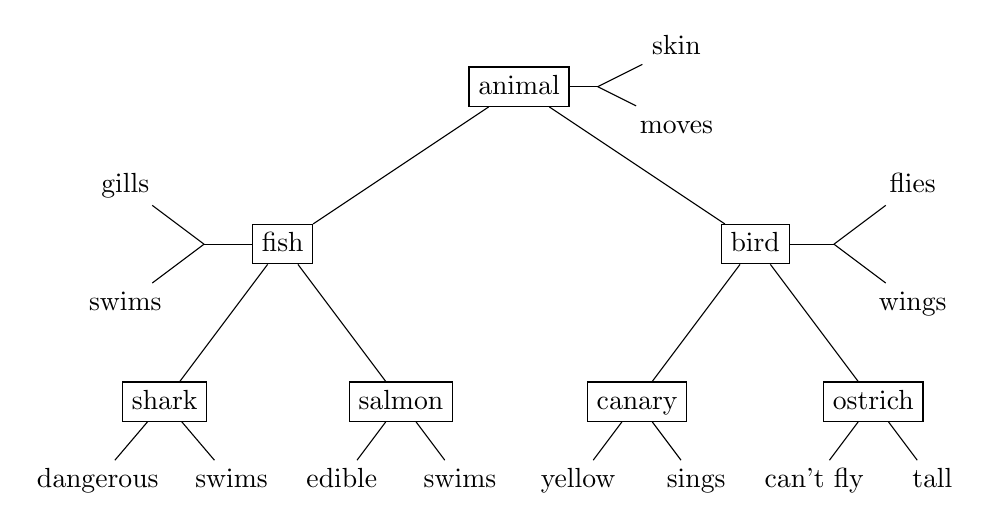
\begin{tikzpicture}[level distance=2cm]
\tikzstyle{every node}=[rectangle,text centered, text height=1.5ex, text depth=0.25ex]
\tikzstyle{category} = [draw];
\node[category] {animal}[sibling distance=3cm]
[grow=down]
child {node[category] {fish}[sibling distance=1.5cm]
  child {node[category] {shark}
     child[level distance=1cm, sibling distance=1.7cm] {node {dangerous}}
     child[level distance=1cm, sibling distance=1.7cm] {node {swims}}}
child[grow=left, level distance=1cm] {
     child {node {gills}}
     child {node {swims}} 
  }
  child {node[category] {salmon}
     child[level distance=1cm, sibling distance=1.5cm] {node {edible}}
     child[level distance=1cm, sibling distance=1.5cm] {node {swims}}
}
}
child[grow=right, sibling distance=1cm, level distance=1cm] {
child {node {moves}}
child {node {skin}}
}
child{node[category] {bird}[sibling distance=1.5cm]
  child {node[category] {canary}
     child[level distance=1cm, sibling distance=1.5cm] {node {yellow}}
     child[level distance=1cm, sibling distance=1.5cm] {node {sings}}
   }
  child[grow=right, level distance=1cm] {
    child {node {wings}}
    child {node {flies}}
  }
  child[level distance=2cm] {node[category] {ostrich}
      child[level distance=1cm, sibling distance=1.5cm] {node {can't fly}}
     child[level distance=1cm, sibling distance=1.5cm] {node {tall}}
  }
};
\end{tikzpicture}
\caption{An example taxonomy of categories and properties. The categories are marked by rectangles, the pure text nodes in the tree are properties. For example, a \emph{shark} is member of the category \emph{fish} and has the direct properties \emph{dangerous} and \emph{swims} and inherits the properties \emph{gills}, \emph{swims}, \emph{moves} and \emph{skin} from its parent categories.}
\label{fig:semantic_model_example}
\end{figure}

Chunks, which encode a property of an object have the form as illustrated in figure~\ref{fig:semantic_model_example:chunks:property}: Each property chunk has a slot \emph{object} which encodes the name of the object. The slot \emph{attribute} holds the name of the attribute like for example \emph{dangerous} or \emph{locomotion}. In the \emph{value} slot, the value of the attribute is defined. The value of the attribute \emph{locomotion} is \emph{swimming} in this example. The chunk in figure~\ref{fig:semantic_model_example:chunks:category} encodes the membership of the object \emph{shark} in the category \emph{fish}. 

\begin{figure}[htb]
\centering
\tikzstyle{chunk} = [ellipse, draw]
\tikzstyle{element} = [] 
\tikzstyle{slot} = [draw, -latex]   
\subfigure[]{
\begin{tikzpicture}[node distance = 2cm, auto]
 \node[chunk] (p1) {\parbox{1.5cm}{\centering p1:\\ property}}; 
 \node[element, left of=p1, node distance=3cm] (object) {shark}; 
 \node[element, above of=p1] (attribute) {dangerous}; 
 \node[element, below of=p1, node distance=2cm] (value) {true}; 

    % Draw edges
  \path[slot] (p1) -- node[above] {object} (object);
  \path[slot] (p1) -- node {attribute} (attribute);
  \path[slot] (p1) -- node {value} (value);
\end{tikzpicture}
\label{fig:semantic_model_example:chunks:property}
}
\qquad
\subfigure[]{
\begin{tikzpicture}[node distance = 2cm, auto]
 \node[chunk] (p3) {\parbox{1.5cm}{\centering p3:\\ property}}; 
 \node[element, left of=p3, node distance=3cm] (object) {shark}; 
 \node[element, above of=p3] (attribute) {category}; 
 \node[element, below of=p3, node distance=2cm] (value) {fish}; 

    % Draw edges
  \path[slot] (p3) -- node[above] {object} (object);
  \path[slot] (p3) -- node {attribute} (attribute);
  \path[slot] (p3) -- node {value} (value);
\end{tikzpicture}
\label{fig:semantic_model_example:chunks:category}
}
\caption{Two chunks of the type \emph{property} encoding properties of the object \emph{shark} as defined in figure~\ref{fig:semantic_model_example}. \subref{fig:semantic_model_example:chunks:property} This chunk encodes the fact, that a shark is dangerous. \subref{fig:semantic_model_example:chunks:category} The membership of an object in a category is also encoded by a \emph{property} chunk. The attribute for this category membership property is \emph{category} and the value encodes the name of the \emph{category}.}
\label{fig:semantic_model_example:chunks}
\end{figure}


To answer a query like ``Is a canary an animal?'' which cannot be answered directly from a \emph{property} chunk, the model must support a recursive search in the tree. The full model code and translation can be found in appendix~\ref{app:ex:semantic_model}. The model uses the concept of duplicate slot tests as described in section~\ref{implementation:duplicate_slot_tests} (see page~\pageref{implementation:duplicate_slot_tests}). However, the compiler cannot handle those tests in the current version and hence the compiled model has to be edited using the pattern from section~\ref{implementation:duplicate_slot_tests}:

\begin{lstlisting}
=retrieval>
      ISA         property
      object      =obj1
      attribute   category
      value       =obj2
    - value       =cat 
\end{lstlisting}

has to be translated to:

\begin{lstlisting}
chain-category@
  buffer(goal,_,A),
    chunk(A,is-member),
    chunk_has_slot(A,object,C),
    chunk_has_slot(A,category,D),
    chunk_has_slot(A,judgment,pending),
  buffer(retrieval,_,B),
    chunk(B,property),
    chunk_has_slot(B,object,C),
    chunk_has_slot(B,attribute,category),
    chunk_has_slot(B,value,E)
  \ apply_rule(chain-category) 
<=> 
  C\==nil,
  D\==nil,
  E\==nil,
  E\==D |
  ...
\end{lstlisting}

I.e., the duplicate slot test for the slot \lstinline|value| is reduced to one single head constraint (\lstinline|chunk_has_slot(B,value,E)|) and a guard, which states that \lstinline|=obj2| $\neq$ \lstinline|=cat| (the built-in check \lstinline|E \== D|). After this small change, the model can be run with various queries, i.e. goal chunks as described in \cite[unit 1, pp. 24\psqq]{actr_tutorial} and appendix~\ref{app:ex:semantic_model}.

%\section{The Fan Model}

%simplified version of fan model